% Created by tikzDevice version 0.12 on 2019-07-24 15:29:03
% !TEX encoding = UTF-8 Unicode
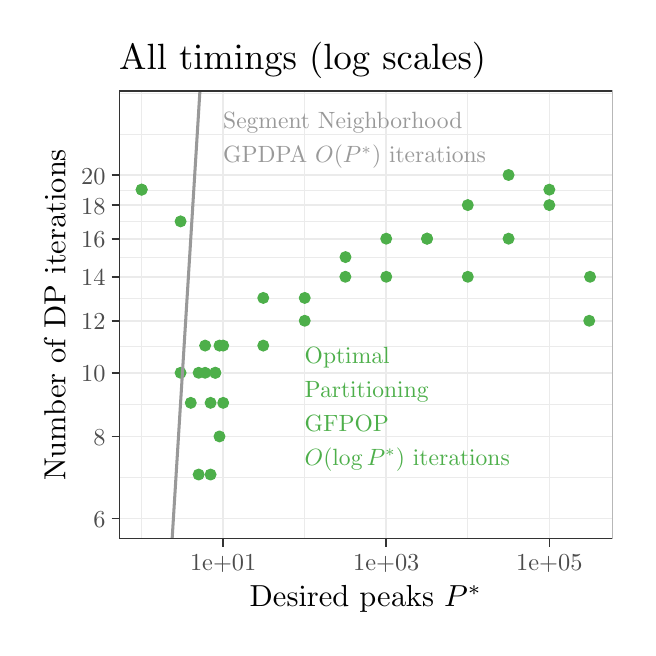
\begin{tikzpicture}[x=1pt,y=1pt]
\definecolor{fillColor}{RGB}{255,255,255}
\path[use as bounding box,fill=fillColor,fill opacity=0.00] (0,0) rectangle (216.81,216.81);
\begin{scope}
\path[clip] (  0.00,  0.00) rectangle (216.81,216.81);
\definecolor{drawColor}{RGB}{255,255,255}
\definecolor{fillColor}{RGB}{255,255,255}

\path[draw=drawColor,line width= 0.6pt,line join=round,line cap=round,fill=fillColor] (  0.00,  0.00) rectangle (216.81,216.81);
\end{scope}
\begin{scope}
\path[clip] ( 33.09, 32.08) rectangle (211.31,193.93);
\definecolor{fillColor}{RGB}{255,255,255}

\path[fill=fillColor] ( 33.09, 32.08) rectangle (211.31,193.93);
\definecolor{drawColor}{gray}{0.92}

\path[draw=drawColor,line width= 0.3pt,line join=round] ( 33.09, 54.27) --
	(211.31, 54.27);

\path[draw=drawColor,line width= 0.3pt,line join=round] ( 33.09, 80.60) --
	(211.31, 80.60);

\path[draw=drawColor,line width= 0.3pt,line join=round] ( 33.09,101.50) --
	(211.31,101.50);

\path[draw=drawColor,line width= 0.3pt,line join=round] ( 33.09,118.85) --
	(211.31,118.85);

\path[draw=drawColor,line width= 0.3pt,line join=round] ( 33.09,133.68) --
	(211.31,133.68);

\path[draw=drawColor,line width= 0.3pt,line join=round] ( 33.09,146.63) --
	(211.31,146.63);

\path[draw=drawColor,line width= 0.3pt,line join=round] ( 33.09,158.14) --
	(211.31,158.14);

\path[draw=drawColor,line width= 0.3pt,line join=round] ( 33.09,178.40) --
	(211.31,178.40);

\path[draw=drawColor,line width= 0.3pt,line join=round] ( 33.09,193.23) --
	(211.31,193.23);

\path[draw=drawColor,line width= 0.3pt,line join=round] ( 41.19, 32.08) --
	( 41.19,193.93);

\path[draw=drawColor,line width= 0.3pt,line join=round] (100.11, 32.08) --
	(100.11,193.93);

\path[draw=drawColor,line width= 0.3pt,line join=round] (159.04, 32.08) --
	(159.04,193.93);

\path[draw=drawColor,line width= 0.6pt,line join=round] ( 33.09, 39.44) --
	(211.31, 39.44);

\path[draw=drawColor,line width= 0.6pt,line join=round] ( 33.09, 69.10) --
	(211.31, 69.10);

\path[draw=drawColor,line width= 0.6pt,line join=round] ( 33.09, 92.10) --
	(211.31, 92.10);

\path[draw=drawColor,line width= 0.6pt,line join=round] ( 33.09,110.90) --
	(211.31,110.90);

\path[draw=drawColor,line width= 0.6pt,line join=round] ( 33.09,126.79) --
	(211.31,126.79);

\path[draw=drawColor,line width= 0.6pt,line join=round] ( 33.09,140.56) --
	(211.31,140.56);

\path[draw=drawColor,line width= 0.6pt,line join=round] ( 33.09,152.70) --
	(211.31,152.70);

\path[draw=drawColor,line width= 0.6pt,line join=round] ( 33.09,163.57) --
	(211.31,163.57);

\path[draw=drawColor,line width= 0.6pt,line join=round] ( 70.65, 32.08) --
	( 70.65,193.93);

\path[draw=drawColor,line width= 0.6pt,line join=round] (129.58, 32.08) --
	(129.58,193.93);

\path[draw=drawColor,line width= 0.6pt,line join=round] (188.50, 32.08) --
	(188.50,193.93);
\definecolor{drawColor}{RGB}{77,175,74}
\definecolor{fillColor}{RGB}{77,175,74}

\path[draw=drawColor,line width= 0.4pt,line join=round,line cap=round,fill=fillColor] ( 41.19,158.28) circle (  1.96);

\path[draw=drawColor,line width= 0.4pt,line join=round,line cap=round,fill=fillColor] ( 55.25, 92.10) circle (  1.96);

\path[draw=drawColor,line width= 0.4pt,line join=round,line cap=round,fill=fillColor] ( 58.93, 81.24) circle (  1.96);

\path[draw=drawColor,line width= 0.4pt,line join=round,line cap=round,fill=fillColor] ( 61.78, 92.10) circle (  1.96);

\path[draw=drawColor,line width= 0.4pt,line join=round,line cap=round,fill=fillColor] ( 64.12,101.93) circle (  1.96);

\path[draw=drawColor,line width= 0.4pt,line join=round,line cap=round,fill=fillColor] ( 66.09, 55.33) circle (  1.96);

\path[draw=drawColor,line width= 0.4pt,line join=round,line cap=round,fill=fillColor] ( 67.80, 92.10) circle (  1.96);

\path[draw=drawColor,line width= 0.4pt,line join=round,line cap=round,fill=fillColor] ( 69.31,101.93) circle (  1.96);

\path[draw=drawColor,line width= 0.4pt,line join=round,line cap=round,fill=fillColor] ( 70.65, 81.24) circle (  1.96);

\path[draw=drawColor,line width= 0.4pt,line join=round,line cap=round,fill=fillColor] ( 85.13,119.15) circle (  1.96);

\path[draw=drawColor,line width= 0.4pt,line join=round,line cap=round,fill=fillColor] (100.11,110.90) circle (  1.96);

\path[draw=drawColor,line width= 0.4pt,line join=round,line cap=round,fill=fillColor] (114.84,133.91) circle (  1.96);

\path[draw=drawColor,line width= 0.4pt,line join=round,line cap=round,fill=fillColor] (129.56,140.56) circle (  1.96);

\path[draw=drawColor,line width= 0.4pt,line join=round,line cap=round,fill=fillColor] (144.31,140.56) circle (  1.96);

\path[draw=drawColor,line width= 0.4pt,line join=round,line cap=round,fill=fillColor] (159.04,152.70) circle (  1.96);

\path[draw=drawColor,line width= 0.4pt,line join=round,line cap=round,fill=fillColor] (173.77,163.57) circle (  1.96);

\path[draw=drawColor,line width= 0.4pt,line join=round,line cap=round,fill=fillColor] (188.50,152.70) circle (  1.96);

\path[draw=drawColor,line width= 0.4pt,line join=round,line cap=round,fill=fillColor] (203.21,126.79) circle (  1.96);

\path[draw=drawColor,line width= 0.4pt,line join=round,line cap=round,fill=fillColor] ( 41.19,158.28) circle (  1.96);

\path[draw=drawColor,line width= 0.4pt,line join=round,line cap=round,fill=fillColor] ( 55.25,146.81) circle (  1.96);

\path[draw=drawColor,line width= 0.4pt,line join=round,line cap=round,fill=fillColor] ( 61.78, 55.33) circle (  1.96);

\path[draw=drawColor,line width= 0.4pt,line join=round,line cap=round,fill=fillColor] ( 64.12, 92.10) circle (  1.96);

\path[draw=drawColor,line width= 0.4pt,line join=round,line cap=round,fill=fillColor] ( 66.09, 81.24) circle (  1.96);

\path[draw=drawColor,line width= 0.4pt,line join=round,line cap=round,fill=fillColor] ( 67.80, 92.10) circle (  1.96);

\path[draw=drawColor,line width= 0.4pt,line join=round,line cap=round,fill=fillColor] ( 69.31, 69.10) circle (  1.96);

\path[draw=drawColor,line width= 0.4pt,line join=round,line cap=round,fill=fillColor] ( 70.65,101.93) circle (  1.96);

\path[draw=drawColor,line width= 0.4pt,line join=round,line cap=round,fill=fillColor] ( 85.13,101.93) circle (  1.96);

\path[draw=drawColor,line width= 0.4pt,line join=round,line cap=round,fill=fillColor] (100.11,119.15) circle (  1.96);

\path[draw=drawColor,line width= 0.4pt,line join=round,line cap=round,fill=fillColor] (114.80,126.79) circle (  1.96);

\path[draw=drawColor,line width= 0.4pt,line join=round,line cap=round,fill=fillColor] (129.58,126.79) circle (  1.96);

\path[draw=drawColor,line width= 0.4pt,line join=round,line cap=round,fill=fillColor] (144.31,140.56) circle (  1.96);

\path[draw=drawColor,line width= 0.4pt,line join=round,line cap=round,fill=fillColor] (159.04,126.79) circle (  1.96);

\path[draw=drawColor,line width= 0.4pt,line join=round,line cap=round,fill=fillColor] (173.77,140.56) circle (  1.96);

\path[draw=drawColor,line width= 0.4pt,line join=round,line cap=round,fill=fillColor] (188.50,158.28) circle (  1.96);

\path[draw=drawColor,line width= 0.4pt,line join=round,line cap=round,fill=fillColor] (202.92,110.90) circle (  1.96);
\definecolor{drawColor}{gray}{0.60}

\path[draw=drawColor,line width= 1.1pt,line join=round] ( 50.21,  0.00) -- ( 63.66,216.81);

\node[text=drawColor,anchor=base west,inner sep=0pt, outer sep=0pt, scale=  0.85] at ( 70.65,180.26) {Segment Neighborhood};

\node[text=drawColor,anchor=base west,inner sep=0pt, outer sep=0pt, scale=  0.85] at ( 70.65,167.97) {GPDPA $O(P^*)$ iterations};

\node[text=drawColor,anchor=base west,inner sep=0pt, outer sep=0pt, scale=  0.85] at ( 70.65,155.68) {};

\node[text=drawColor,anchor=base west,inner sep=0pt, outer sep=0pt, scale=  0.85] at ( 70.65,143.39) {};
\definecolor{drawColor}{RGB}{77,175,74}

\node[text=drawColor,anchor=base west,inner sep=0pt, outer sep=0pt, scale=  0.85] at (100.11, 95.62) {Optimal};

\node[text=drawColor,anchor=base west,inner sep=0pt, outer sep=0pt, scale=  0.85] at (100.11, 83.33) {Partitioning};

\node[text=drawColor,anchor=base west,inner sep=0pt, outer sep=0pt, scale=  0.85] at (100.11, 71.04) {GFPOP};

\node[text=drawColor,anchor=base west,inner sep=0pt, outer sep=0pt, scale=  0.85] at (100.11, 58.75) {$O(\log P^*)$ iterations};
\definecolor{drawColor}{gray}{0.20}

\path[draw=drawColor,line width= 0.6pt,line join=round,line cap=round] ( 33.09, 32.08) rectangle (211.31,193.93);
\end{scope}
\begin{scope}
\path[clip] (  0.00,  0.00) rectangle (216.81,216.81);
\definecolor{drawColor}{gray}{0.30}

\node[text=drawColor,anchor=base east,inner sep=0pt, outer sep=0pt, scale=  0.88] at ( 28.14, 36.19) {6};

\node[text=drawColor,anchor=base east,inner sep=0pt, outer sep=0pt, scale=  0.88] at ( 28.14, 65.85) {8};

\node[text=drawColor,anchor=base east,inner sep=0pt, outer sep=0pt, scale=  0.88] at ( 28.14, 88.85) {10};

\node[text=drawColor,anchor=base east,inner sep=0pt, outer sep=0pt, scale=  0.88] at ( 28.14,107.65) {12};

\node[text=drawColor,anchor=base east,inner sep=0pt, outer sep=0pt, scale=  0.88] at ( 28.14,123.54) {14};

\node[text=drawColor,anchor=base east,inner sep=0pt, outer sep=0pt, scale=  0.88] at ( 28.14,137.31) {16};

\node[text=drawColor,anchor=base east,inner sep=0pt, outer sep=0pt, scale=  0.88] at ( 28.14,149.45) {18};

\node[text=drawColor,anchor=base east,inner sep=0pt, outer sep=0pt, scale=  0.88] at ( 28.14,160.31) {20};
\end{scope}
\begin{scope}
\path[clip] (  0.00,  0.00) rectangle (216.81,216.81);
\definecolor{drawColor}{gray}{0.20}

\path[draw=drawColor,line width= 0.6pt,line join=round] ( 30.34, 39.44) --
	( 33.09, 39.44);

\path[draw=drawColor,line width= 0.6pt,line join=round] ( 30.34, 69.10) --
	( 33.09, 69.10);

\path[draw=drawColor,line width= 0.6pt,line join=round] ( 30.34, 92.10) --
	( 33.09, 92.10);

\path[draw=drawColor,line width= 0.6pt,line join=round] ( 30.34,110.90) --
	( 33.09,110.90);

\path[draw=drawColor,line width= 0.6pt,line join=round] ( 30.34,126.79) --
	( 33.09,126.79);

\path[draw=drawColor,line width= 0.6pt,line join=round] ( 30.34,140.56) --
	( 33.09,140.56);

\path[draw=drawColor,line width= 0.6pt,line join=round] ( 30.34,152.70) --
	( 33.09,152.70);

\path[draw=drawColor,line width= 0.6pt,line join=round] ( 30.34,163.57) --
	( 33.09,163.57);
\end{scope}
\begin{scope}
\path[clip] (  0.00,  0.00) rectangle (216.81,216.81);
\definecolor{drawColor}{gray}{0.20}

\path[draw=drawColor,line width= 0.6pt,line join=round] ( 70.65, 29.33) --
	( 70.65, 32.08);

\path[draw=drawColor,line width= 0.6pt,line join=round] (129.58, 29.33) --
	(129.58, 32.08);

\path[draw=drawColor,line width= 0.6pt,line join=round] (188.50, 29.33) --
	(188.50, 32.08);
\end{scope}
\begin{scope}
\path[clip] (  0.00,  0.00) rectangle (216.81,216.81);
\definecolor{drawColor}{gray}{0.30}

\node[text=drawColor,anchor=base,inner sep=0pt, outer sep=0pt, scale=  0.88] at ( 70.65, 20.63) {1e+01};

\node[text=drawColor,anchor=base,inner sep=0pt, outer sep=0pt, scale=  0.88] at (129.58, 20.63) {1e+03};

\node[text=drawColor,anchor=base,inner sep=0pt, outer sep=0pt, scale=  0.88] at (188.50, 20.63) {1e+05};
\end{scope}
\begin{scope}
\path[clip] (  0.00,  0.00) rectangle (216.81,216.81);
\definecolor{drawColor}{RGB}{0,0,0}

\node[text=drawColor,anchor=base,inner sep=0pt, outer sep=0pt, scale=  1.10] at (122.20,  7.62) {Desired peaks $P^*$};
\end{scope}
\begin{scope}
\path[clip] (  0.00,  0.00) rectangle (216.81,216.81);
\definecolor{drawColor}{RGB}{0,0,0}

\node[text=drawColor,rotate= 90.00,anchor=base,inner sep=0pt, outer sep=0pt, scale=  1.10] at ( 13.63,113.01) {Number of DP iterations};
\end{scope}
\begin{scope}
\path[clip] (  0.00,  0.00) rectangle (216.81,216.81);
\definecolor{drawColor}{RGB}{0,0,0}

\node[text=drawColor,anchor=base west,inner sep=0pt, outer sep=0pt, scale=  1.32] at ( 33.09,201.55) {All timings (log scales)};
\end{scope}
\end{tikzpicture}
